\documentclass[11pt, a4paper,twocolumn]{jarticle}
\usepackage[dvipdfmx]{graphicx}

\begin{document}
%=============================================================
\section{Making electric circuits for capturing sound waves (microphone) and emitting sound waves (speaker) ($3^{rd} day$)}
% ===============================================================
\subsection{Purpose}
今回の実験では電気回路を作りその回路を使い,音声を電気信号に変えたり逆に電気信号を音声に変える方法を学ぶことが目的である.
% =======================================================
\subsection{Procedure}
\noindent
\textbf{Task 3.1} \\
まず音声信号を電気信号に変換するための電気回路を作る.図\ref{fig:15}に示されるように電気回路を製作する.
この際プリント基板に半田付けして回路を実装する.

\begin{figure}[htbp]
 \begin{center}
  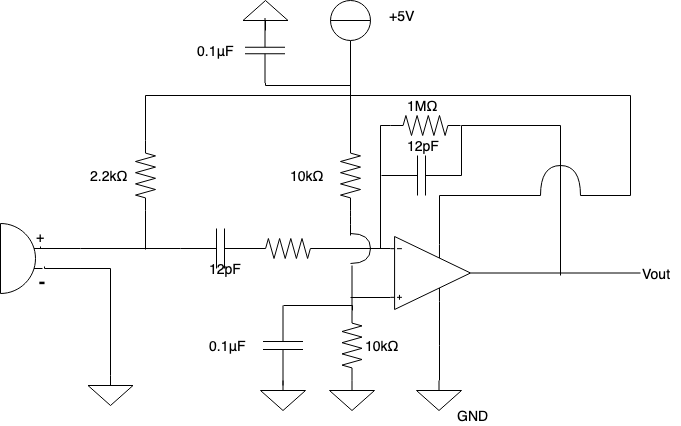
\includegraphics[width=0.8\linewidth]{fig15.png}
 \end{center}
 \caption{capture回路}
 \label{fig:15}
\end{figure}

\noindent
\textbf{Task 3.2} \\
先ほどの実験で作ったcapture回路をAD/DA変換機に接続しCプログラムにより音叉の音声データを取得する.この際にサンプリング定理に気をつけて音波を測定する.また回路の都合上出力電圧が2.5V付近を中心に0Vから5Vの間を振動することに気をつける.
取得したデータをテキストファイルとして保存する.
また今回の実験ではデータ数を1000,サンプリング周波数を10kHzとして測定をおこなった.

\noindent
\textbf{Task 3.3} \\
次にデジタル信号を音声に変換するためのスピーカーを作る.図\ref{fig:16}に示すようにスピーカー回路を作る.
その後Cプログラムにより作った正弦波を出力し音波を発生させる.
さらに周波数が近いと同時に鳴らすことによりうなりを観測する.
この際入力電圧は0Vを中心として電圧を入力することに注意する.

\begin{figure}[htbp]
 \begin{center}
  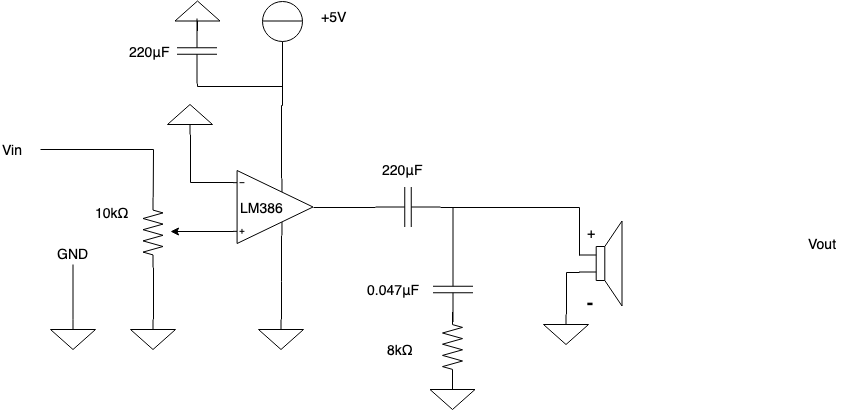
\includegraphics[width=0.8\linewidth]{fig16.png}
 \end{center}
 \caption{speaker回路}
 \label{fig:16}
\end{figure}

\noindent
\textbf{Task 3.4} \\
マイクを用いて声を録音し,録音時と同じサンプリング周波数,データ数で再生し正しく再生できたかを確認する.
次にサンプリング周波数を録音時のサンプリング周波数とくらべ2倍,3倍にして声がどのように変化したのかを確認する.
この際データ数を20000点,サンプリング周波数を20kHzとして「こんにちは」という声の測定を行なった.
% =======================================================
\subsection{Result}
\noindent
\textbf{Task 3.1 電気回路の作成} \\
今回はマイク回路がうまく作ることができなかったので既製品を使用した.
スピーカー回路に関しては正弦波を入力とし音を鳴らすことで動作を確認した.

\noindent
\textbf{Task 3.2} \\
実験より以下の図に示すような波形を得た.

\begin{figure}[htbp]
 \begin{center}
  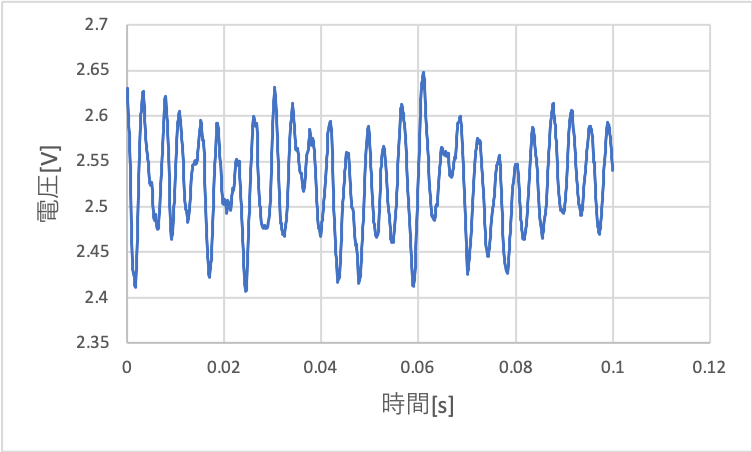
\includegraphics[width=0.8\linewidth]{fig17.png}
 \end{center}
 \caption{262Hz音叉}
 \label{fig:17}
\end{figure}

\begin{figure}[htbp]
 \begin{center}
  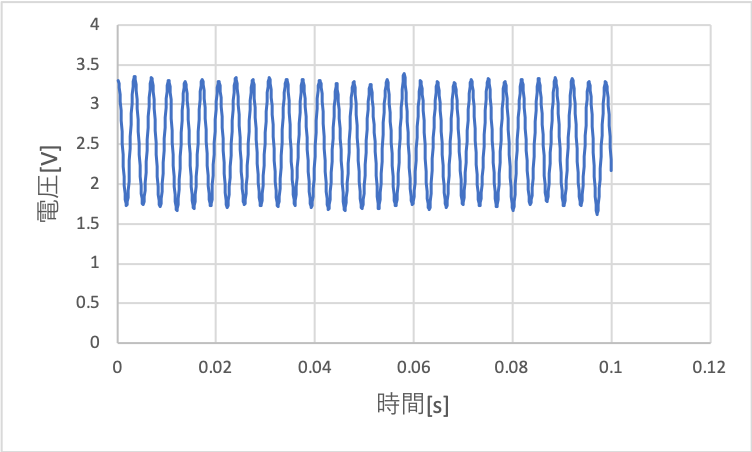
\includegraphics[width=0.8\linewidth]{fig18.png}
 \end{center}
 \caption{294Hz音叉}
 \label{fig:18}
\end{figure}

\begin{figure}[htbp]
 \begin{center}
  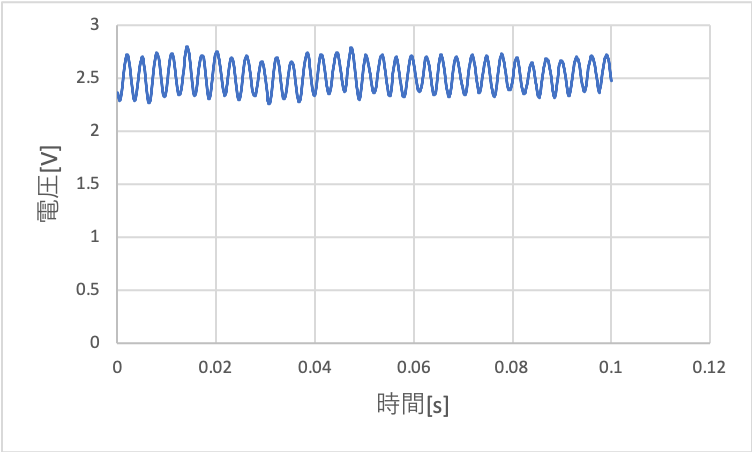
\includegraphics[width=0.8\linewidth]{fig19.png}
 \end{center}
 \caption{330Hz音叉}
 \label{fig:19}
\end{figure}

\begin{figure}[htbp]
 \begin{center}
  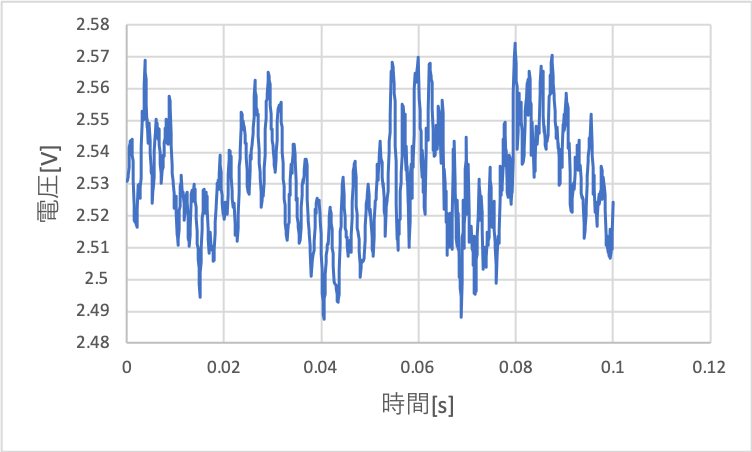
\includegraphics[width=0.8\linewidth]{fig20.png}
 \end{center}
 \caption{392Hz音叉}
 \label{fig:20}
\end{figure}

\begin{figure}[htbp]
 \begin{center}
  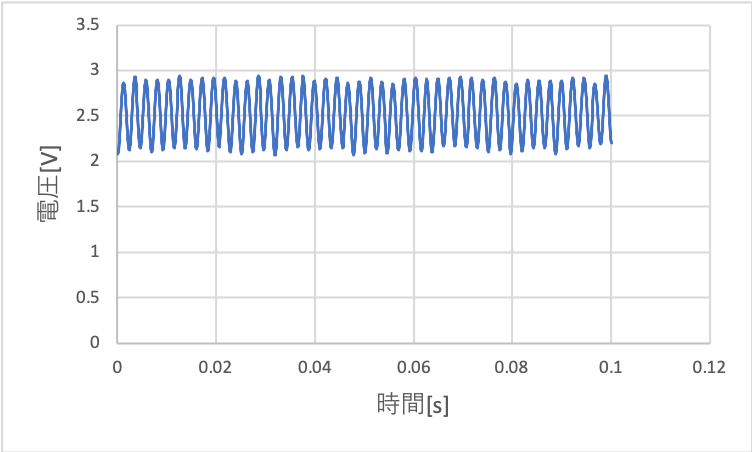
\includegraphics[width=0.8\linewidth]{fig21.png}
 \end{center}
 \caption{440Hz音叉}
 \label{fig:21}
\end{figure}

\noindent
\textbf{Task 3.3} \\
スピーカーで入力正弦波を262Hzから440Hzまでの5種類を順番に再生したところ,再生された音が徐々に高くなっていくことが確認された.
また263Hzの正弦波をプログラムにより作り出しスピーカーで出力し,同時に262Hzの音叉を鳴らしたところ約1秒ごとにうなりを観測できた.

\noindent
\textbf{Task 3.4} \\
測定した際と同じサンプリング周波数,データ点数で音声をスピーカーで再生したところ元の音源と同じ「こんにちは」という音を観測することができた.
また,サンプリング周波数を計測時の2倍,3倍である40kHz,60kHzにしたところ音声は高い声となって再生された.

%============================================================
\subsection{Discussion}
\noindent
\textbf{Task 3.1} \\
マイク回路で取得したデジタル信号をスピーカー回路接続することで適切な音源を得られたのでこれらの回路は正確に昨日していたと考えられる.

\noindent
\textbf{Task 3.2} \\
図\ref{fig:17},\ref{fig:20}図\ref{fig:17}から周囲的な波が得られているので音叉の音波を正確に即てできたと考えられる.
一方図\ref{fig:17},\ref{fig:20}においては波が周期的ではなく振幅もバラバラとなってしまった.
この原因としては測定するタイミングが音叉の振動している範囲に比べて早すぎた,または遅すぎた,また外部の音がノイズとして入り込んだなどが考えられる.

また今回のサンプリング間隔が適切であったかの考察をする.
まずサンプリング定理より\cite{1}サンプリング間隔T,最大周波数$f_M$が満たすべき条件は以下のようになる.
\begin{equation}
    T < \frac{1}{2f_M}
\end{equation}
今回の測定で最大周波数は440Hzであり,サンプリング間隔は$1.0 \times 10^{-4}[s]$であるので明らかに条件を満たしていると考えられる.
したがって今回の実験では適切に量子化できたと考えられる.

\noindent
\textbf{Task 3.3} \\
今回の実験で正弦波の周波数を上げてい行った際にスピーカーから聞こえた音も次第に高くなっていったため適切に出力できたと考えられる.
また二つの正弦波(周波数$f_1$,$f_2$)の合成によるうなり周期Tは以下のように表される.
\begin{equation}
    T = \frac{1}{|f_1-f_2|}
\end{equation}
したがって,263Hzの波を出力した際に262Hzの音叉と約1秒間間隔のうなりが聞こえたことはこの公式より適切であると考えられる.

\noindent
\textbf{Task 3.4} \\
声の測定時はサンプリング周波数は20kHz,データ数は20000個であったので再生する際のサンプリング周波数を測定時と同じ20kHzにした場合測定時と同じ速度で計測した声が再生されたと考えられ実験結果に一致する.
さらに再生時にサンプリング周波数を40kHzにした場合には20kHzで再生した場合に比べて倍速で再生されると考えられる.
その結果再生される声の周波数は2倍となり結果として高い声が出力されたと考えられる.
同様にサンプリング周波数を30kHzにした場合は周波数が3倍となったと考えられる.
逆にサンプリング周波数を10kHzにした場合は周波数が1/2倍されると考えられ低い声が観測されると考えられる.
%=============================================================
\newpage
\end{document}
